\section{Life Cycle Assessment}

% Here is information about figure placement options:
% https://tex.stackexchange.com/questions/35125/how-to-use-the-placement-options-t-h-with-figures

\begin{figure}[htbp]
    \centering
    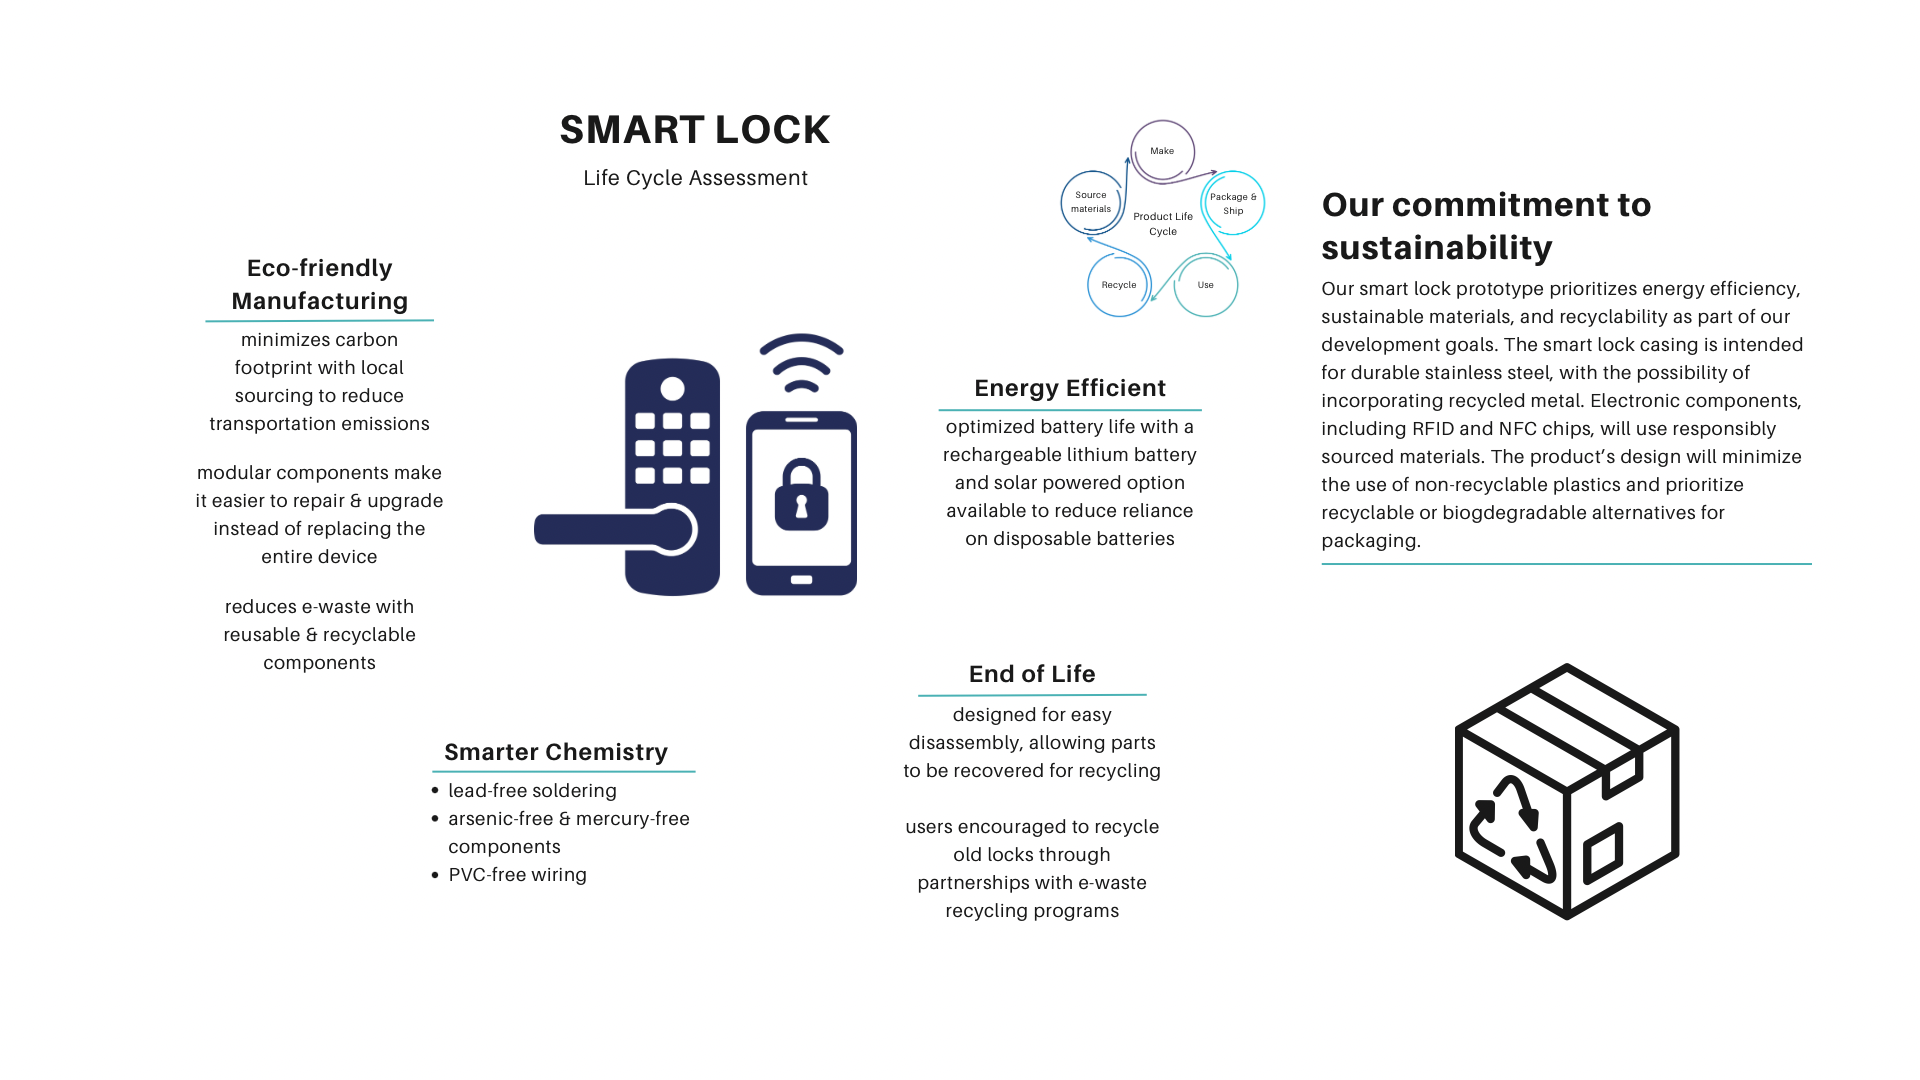
\includegraphics[width=1 \linewidth]{./img/LifeCycleAssessment.png}
    \caption{Smart Lock Life Cycle Assessment}
    \label{fig:LifeCycleFig}
\end{figure}

Adding on to Fig. \ref{fig:LifeCycleFig}, our material usage will be very minimal to what we have already listed in the section \ref{DesignForManufacture}. For the material used on our door lock, we plan to use recycled stainless steel metals (from junk yards) to build the frame of the lock. This allows our product to be easily recyclable without losing any quality of the stainless steel.
